
\title{Lab 1: Filtering Operations}
\author{
        Miquel Marti Rabadan\\921019-1459\\miquelmr@kth.se
}
\date{\today}

\documentclass[12pt]{article}

\usepackage{graphicx,epsfig,palatino,epstopdf}

\begin{document}
\maketitle

%\begin{abstract}
%This is the paper's abstract \ldots
%\end{abstract}

%\section{Introduction}
%This is time for all good men to come to the aid of their party!

\paragraph{Question 1: 
Repeat this exercise with the coordinates p and q set to (5, 9), (9, 5), (17, 9),
(17, 121), (5, 1) and (125, 1) respectively. What do you observe?} 
The first and second coordinate sets, the third and fourth, ... give similar inverse transforms.  The value of p determines the number of periods in the x axis of the IFFT, the value of q the number of periods in the y axis, for the real and imaginary parts and the phase. The amplitude is constant as the inverse Fourier Transform of a delta is a complex exponential.

\paragraph{Question 2:
Explain how a position (p,q) in the Fourier domain will be projected as a sine wave in the spatial domain. Illustrate with a Matlab figure.}
A position (p,q) in the Fourier domain is projected as a complex exponential in the spatial domain, which can be split into real and imaginary part. It can be seen as a basis vector \(e^{j\mathbf{\omega}^T\mathbf{x}}\) being \(\omega\) the vector defining the angular frequencies in x and y directions and \(\mathbf{x}= (x,y)^T\). The angular frequencies \(\omega\) are related to (p,q) as \(\omega=2\pi(p-1,q-1)^T\) when p and q are smaller than half the size of the image. Otherwise, they require the centring done in the second plot in figure \ref{fig:q2} to reorder the quarters of the Fourier transform and have it centred around (0,0).

\begin{figure}[htbp]
 \centering
 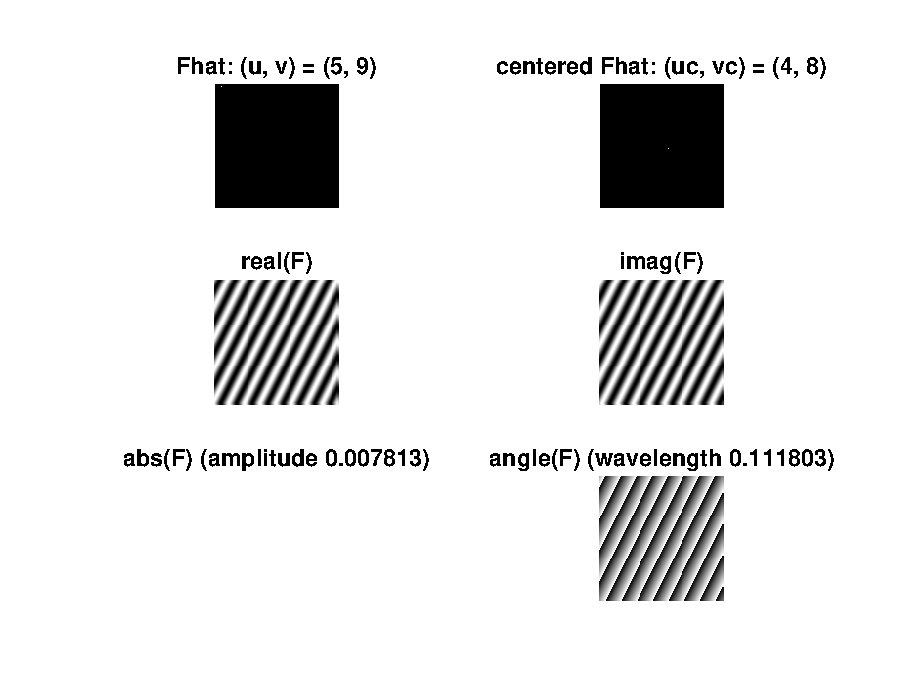
\includegraphics[width=\textwidth]{q2}
 \caption{Basis function representation for \((u,v)=(5,9)\)}
 \label{fig:q2}
\end{figure}

\paragraph{Question 3:
How large is the amplitude? Write down the expression derived from Equation 4 in the notes. Complement the code (variable \(\mathbf{amplitude}\)) accordingly.}
The amplitude is constant and with a value of \(A=\frac{1}{N}=0.0078\) for a image size of 128 samples, as the amplitude of the delta in the Fourier transform is 1. Matlab implementation of the IFFT uses a factor of \(1/N^2\) so the value of the amplitude given has to be multiplied by N.

\paragraph{Question 4: How does the direction and length of the sine wave depend on p and q? Draw an illustrative figure on paper. Write down the explicit expression that can be found in
the lecture notes. Complement the code (variable wavelength) accordingly.}
The direction of the sine wave depends on p and q as \(\alpha=\tan^{-1}(\frac{q}{p})\) being \(\alpha\) the angle of the sine wave direction between the x and y axes, zero for the sine wave direction on the x axis. Figure \ref{fig:q2} shows a sine wave with an angle of 61 degrees above the x axis. The wavelength is defined as the inverse of the Euclidean norm of the vector containing the frequencies for both directions x and y. The wavelength is \(\lambda=\frac{1}{\|(u_c,v_c)\|}\), which is normalized with respect to the image size, for a wavelength value in pixels we should multiply by image size N.

\paragraph{Question 5: What happens when we pass the point in the center and either p or q exceeds half the image size? Explain and illustrate graphically with Matlab.}
These points are then folded into lower values for the frequencies. As done in second plot in Figure \ref{fig:q5}, the point (125,1) is shown centred around (0,0) and corresponds to \((u_c,v_c)=(-4,0)\). This happens because 64 is the maximum frequency that can be represented by an image of size NxN with N=128, that is N/2. Due to sampling, the spectrum represented in the FT image is periodic so it is the same to represent it from frequencies from 0 to N than from -N/2 to N/2, although the second can be interpreted more easily.
\begin{figure}[htbp]
 \centering
 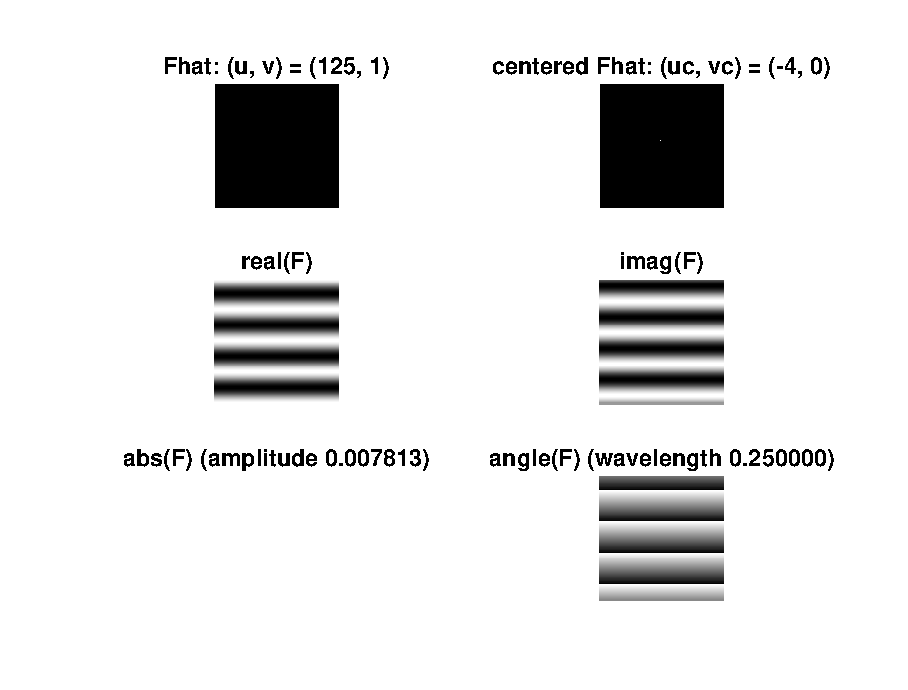
\includegraphics[width=\textwidth]{q5}
 \caption{Basis function representation for \((u,v)=(125,1)\)}
 \label{fig:q5}
\end{figure}

\paragraph{Question 6: What is the purpose of the instructions following the question "What is done
by these instructions?" in the code?} Center the origin, so to have origin in the middle of
the image as [0,0] instead that in the upper left corner as [1,1]. That is equivalent to interchange quarters of the Fourier transform. In this way we are seeing at it as the FT from -N/2 to N/2 instead of from frequencies 0 to N for each of the axis.

\paragraph{Question 7: Why are these Fourier spectra concentrated to the borders of the images? Can you give a mathematical interpretation? Hint: think of the frequencies in the source image and consider the resulting image as a Fourier transform applied to a 2D function. It might be easier to analyse each dimension separately!}
The Fourier spectra are concentrated to the borders of the images as these images contain only frequency zero for one of the axis (there is no variation along it) and a component across all frequencies for the other derived by the box like shape in that axis. Figure \ref{fig:q7_1} shows the differences for the three different images F, G and H and their spectra. F has only variation in the x-axis thus its spectrum has only a component for zero frequency of the y-axis with a sinc-like shape along the x-axis.

\begin{figure}[htbp]
 \centering
 \includegraphics[width=\textwidth]{q7_1}
 \caption{Images F, G and H and their Fourier spectra.}
 \label{fig:q7_1}
\end{figure}

\paragraph{Question 8: Why is the logarithm function applied?}
The logarithm function is applied in order to bring closer the distant values appearing in the Fourier spectrum for a better visualization, reduce the dynamic range of the image spectrum.

\paragraph{Question 9: What conclusions can be drawn regarding linearity? From your observations can you derive a mathematical expression in the general case?}
In image H spectrum, the two other spectra are summed together, proving the linearity of the Fourier transform as it is appears from the sum in the spatial domain. \(\mathcal{F}(aX+bY)=a\mathcal{F}(X)+b\mathcal{F}(Y)\). Figure \ref{fig:q7_2} shows the resulting spectrum of the image sum of F and 2G, shown using the \texttt{fftshift} function that reorders quarters of the Fourier spectrum to have the origin in the middle of the image, similarly to what has been done in Q6.

\begin{figure}[htbp]
 \centering
 \includegraphics[width=\textwidth]{q7_2}
 \caption{Spectrum of F+2G, shown with two different and equivalent functions}
 \label{fig:q7_2}
\end{figure}

\paragraph{Question 10: Are there any other ways to compute the last image? Remember what multiplication in Fourier domain equals to in the spatial domain! Perform these alternative
computations in practice.}
As we are multiplying the two images in the spatial domain that equals to a convolution in the Fourier domain. This equals to \(\hat{F}*\hat{G}\). \(F.*G\), \(\mathcal{F}(F.*G)\) and \(\hat{F}*\hat{G}\) are showed in Figure \ref{fig:q10}. A factor of \(1/N^2\) has to be applied to coincide with the Fourier transform definition. 

\begin{figure}[htbp]
 \centering
 \includegraphics[width=\textwidth]{q10}
 \caption{\(F.*G\), \(\mathcal{F}(F.*G)\) and \(\hat{F}*\hat{G}\).}
 \label{fig:q10}
\end{figure}

\paragraph{Question 11: What conclusions can be drawn from comparing the results with those in the previous exercise? See how the source images have changed and analyze the effects of scaling.}
A compression(expansion) in one axis in the spatial domain gives a expansion(compression) in the same axis in frequency domain. Figure \ref{fig:q11} shows an exampled used to illustrate this statement. The image has been compressed in x-axis and expanded in y-axis. Its spectrum has a narrower main lobe respect the y frequencies and broader respect the x-axis.

\begin{figure}[htbp]
 \centering
 \includegraphics[width=\textwidth]{q11}
 \caption{Scaled version of F and its Fourier spectrum.}
 \label{fig:q11}
\end{figure}

\paragraph{Question 12: What can be said about possible similarities and differences? Hint: think of the frequencies and how they are affected by the rotation.}
The shape of the frequency pattern is the same but has been rotated the same as the original image. In the case of having diagonal lines, the spectrum changes because of the discretization this lines cannot be completely straight.
\begin{figure}[htbp]
 \centering
 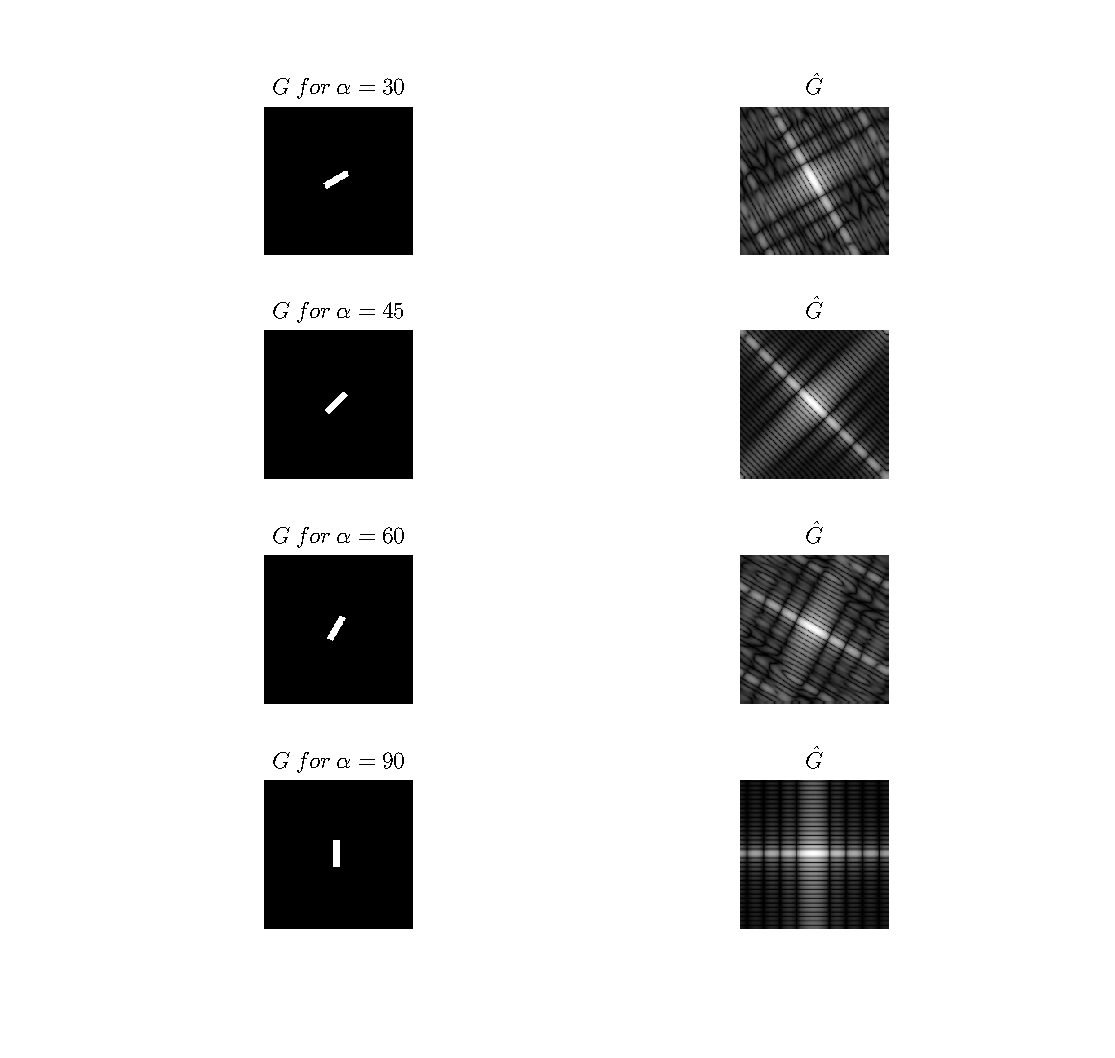
\includegraphics[width=\textwidth]{q12}
 \caption{Rotated versions of F and their Fourier spectra for 30, 45, 60 and 90 degrees rotations.}
 \label{fig:q12}
\end{figure}

\paragraph{Question 13: What information is contained in the phase and in the magnitude of the Fourier transform?}
Phase contains information about the location of the features in the image while magnitude contains information on the shape of those features. In Figure \ref{fig:q13} it can be seen how changing the amplitude produces some effects mainly in changing the intensity of the different elements in the image but still they can be recognized. However, when keeping the magnitude and randomizing the phase the result is a image which cannot be recognized, as the features location has been changed randomly and the final composition is unrecognisable.

\begin{figure}[htbp]
 \centering
 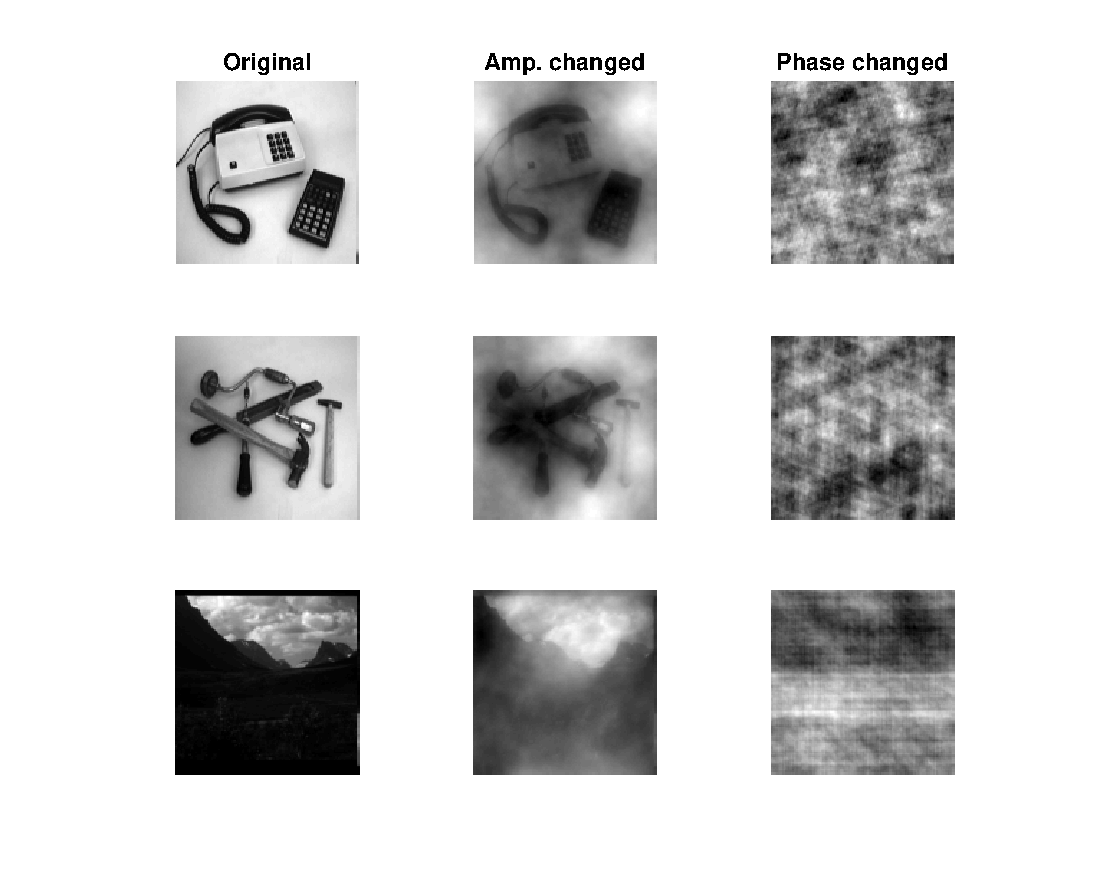
\includegraphics[width=\textwidth]{q13}
 \caption{Images reconstructed after changing amplitude and phase information of its Fourier transforms.}
 \label{fig:q13}
\end{figure}

\paragraph{Question 14: Show the impulse response and variance for the above mentioned t-values. What are the variances of your discretized Gaussian kernel for t = 0.1, 0.3, 1.0, 10.0 and
100.0?}
The impulse responses and variance values are shown in Figure \ref{fig:q14}.

\begin{figure}[htbp]
 \centering
 \includegraphics[width=0.7\textwidth]{q14}
 \caption{Impulse responses for different values of \(t\).}
 \label{fig:q14}
\end{figure}

\paragraph{Question 15: Are the results different from or similar to the estimated variance? How does the result correspond to the ideal continuous case? Lead: think of the relation between spatial and Fourier domains for different values of t.}
They are approximately the same for the higher values of t. For the lower values the Gaussian is represented with a very few number of pixels so the approximation of the continuous Gaussian is bad.

\paragraph{Question 16: Convolve a couple of images with Gaussian functions of different variances
(like t = 1.0, 4.0, 16.0, 64.0 and 256.0) and present your results. What effects can you
observe?}
The convolution with the Gaussian Kernel blurs the image as it works as a low pass filter. For greater values of t, the Fourier spectrum of the kernel is narrower, selecting only lower frequencies. Alternatively it can be seen in the spatial domain, where the impulse response of the kernel is wider for greater values of t so the convolution has a wider support and thus does an "average" over more pixels for each one.

\begin{figure}[htbp]
 \centering
 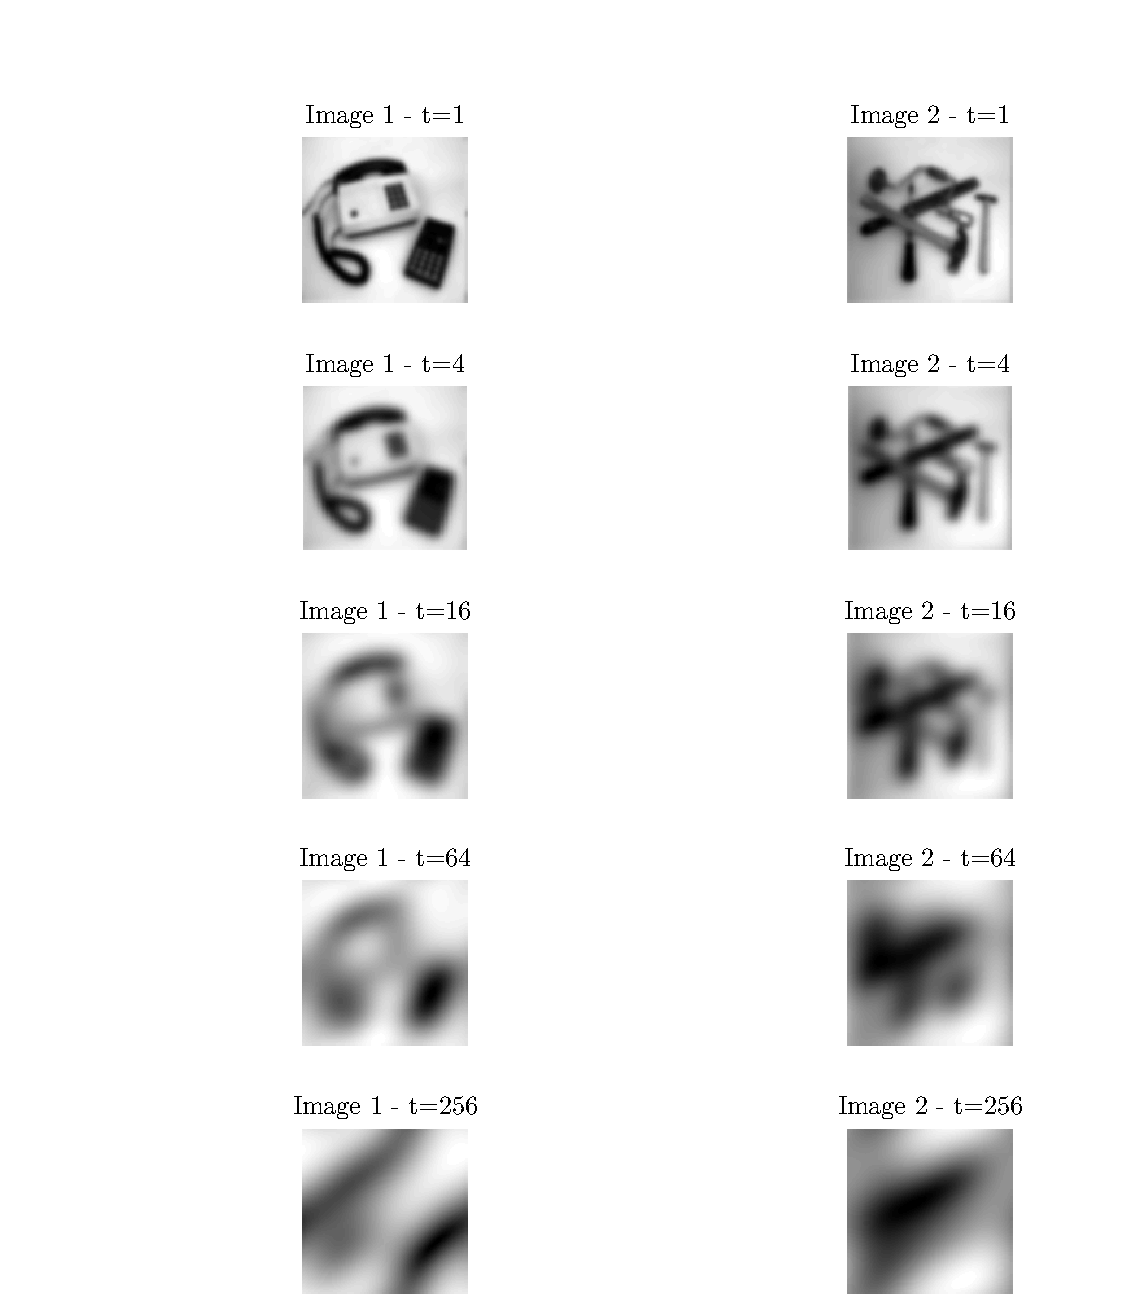
\includegraphics[width=\textwidth]{q16}
 \caption{Image \texttt{phonecalc} and \texttt{few} convolved with the Gaussian kernel for different values of \(t\).}
 \label{fig:q16}
\end{figure}

\paragraph{Question 17: What are the positive and negative effects for each type of filter? Describe what you observe and name the effects that you recognize. How do the results depend on the filter parameters? Illustrate with Matlab figure(s).}
The original image and its versions with white Gaussian noise and salt-and-pepper noise are shown in Figure \ref{fig:q17} with their respective spectra. Figures \ref{fig:q17b} and \ref{fig:q17c} show the filtered versions of the noisy images for the different filters and parameters. The Gauss smoothing filter blurs the image thus removing noise but works better for Gaussian noise. For SAP noise it requires more blur to remove the noisy pixels.
The median filter works better for the SAP noise in which it achieves a complete elimination of the noisy pixels. For the Gaussian noise image it is less effective as all the pixels in the neighbourhood for which the median is computed are affected by some noise. It introduces some artifacts in straight lines and makes the image look like a paint but it preserves the edges.
The ideal low-pass filter removes some noise but creates important "ringing" artifacts, attributed to the Gibbs phenomenon. However, it works better for the Gaussian noise than for the SAP noise.

\begin{figure}[htbp]
 \centering
 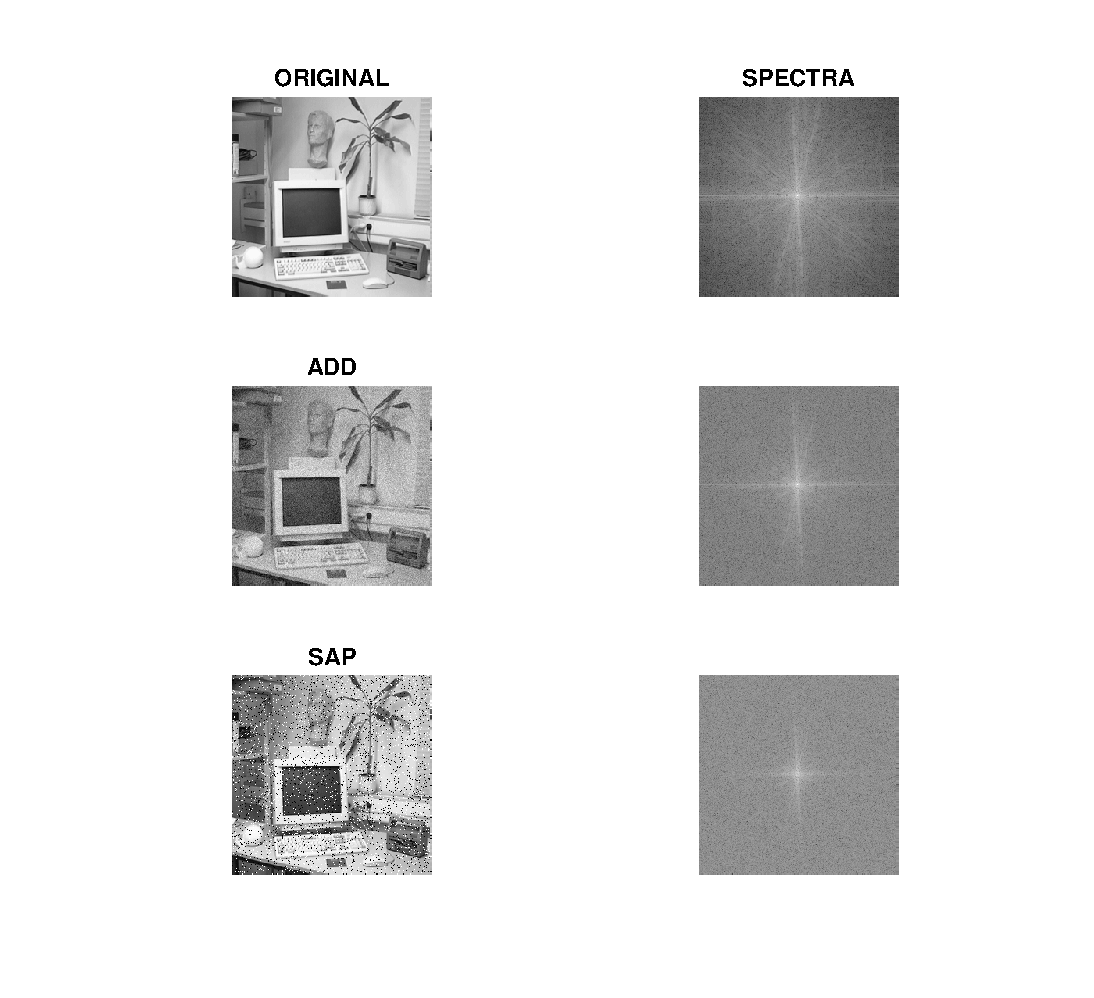
\includegraphics[width=\textwidth]{q17}
 \caption{Image \texttt{office} and versions with added white Gaussian noise and salt-and-peppar noise and their spectra.}
 \label{fig:q17}
\end{figure}

\begin{figure}[htbp]
 \centering
 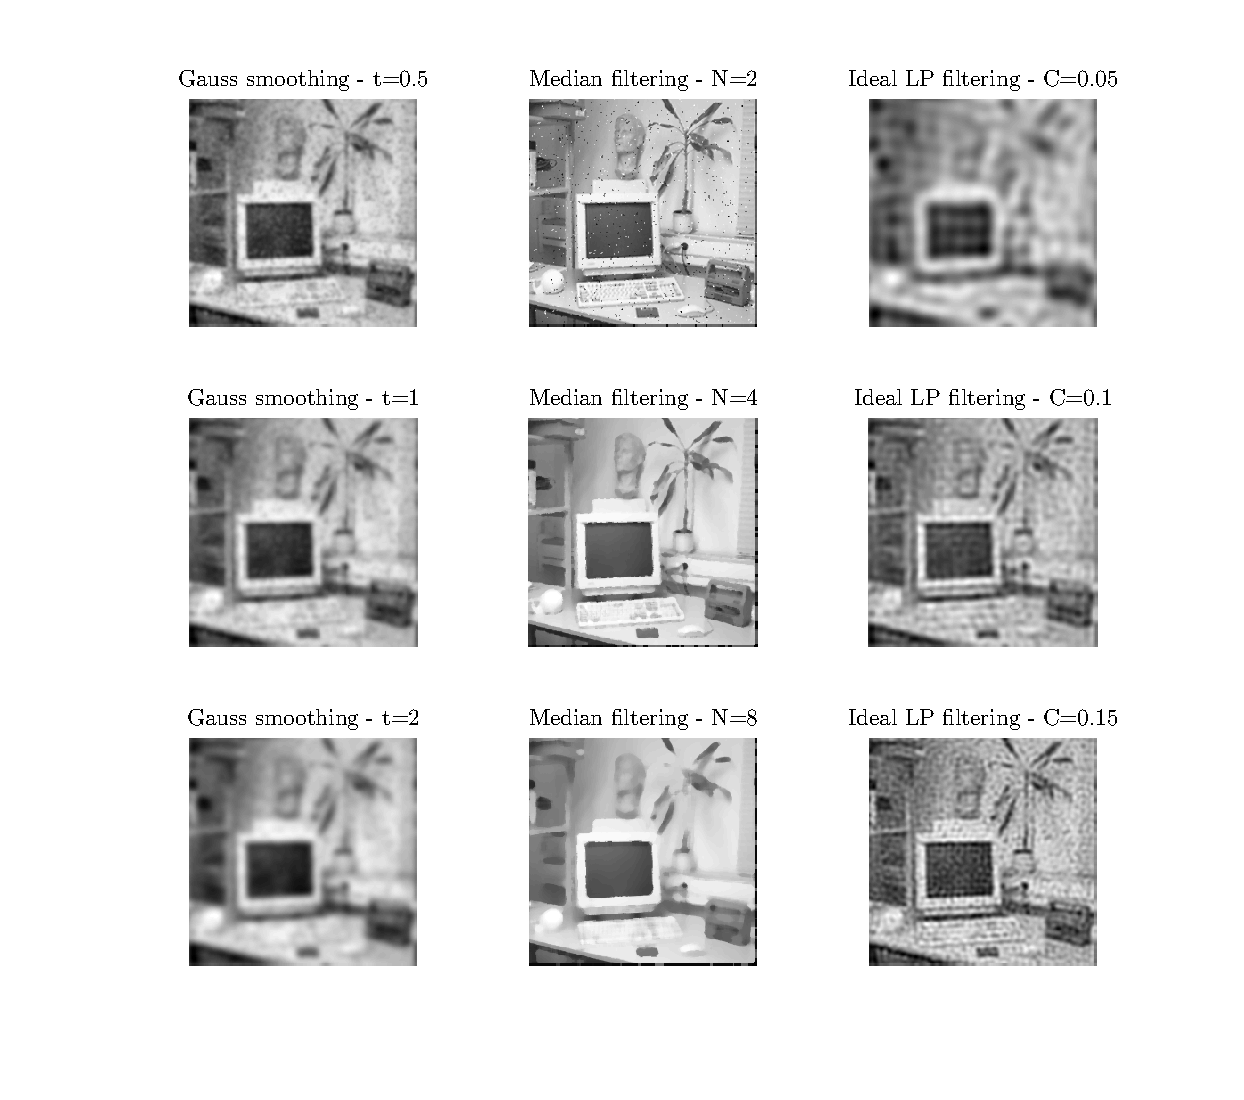
\includegraphics[width=\textwidth]{q17b}
 \caption{Image \texttt{office} with salt-and-peppar noise filtered with different methods and parameters.}
 \label{fig:q17b}
\end{figure}

\begin{figure}[htbp]
 \centering
 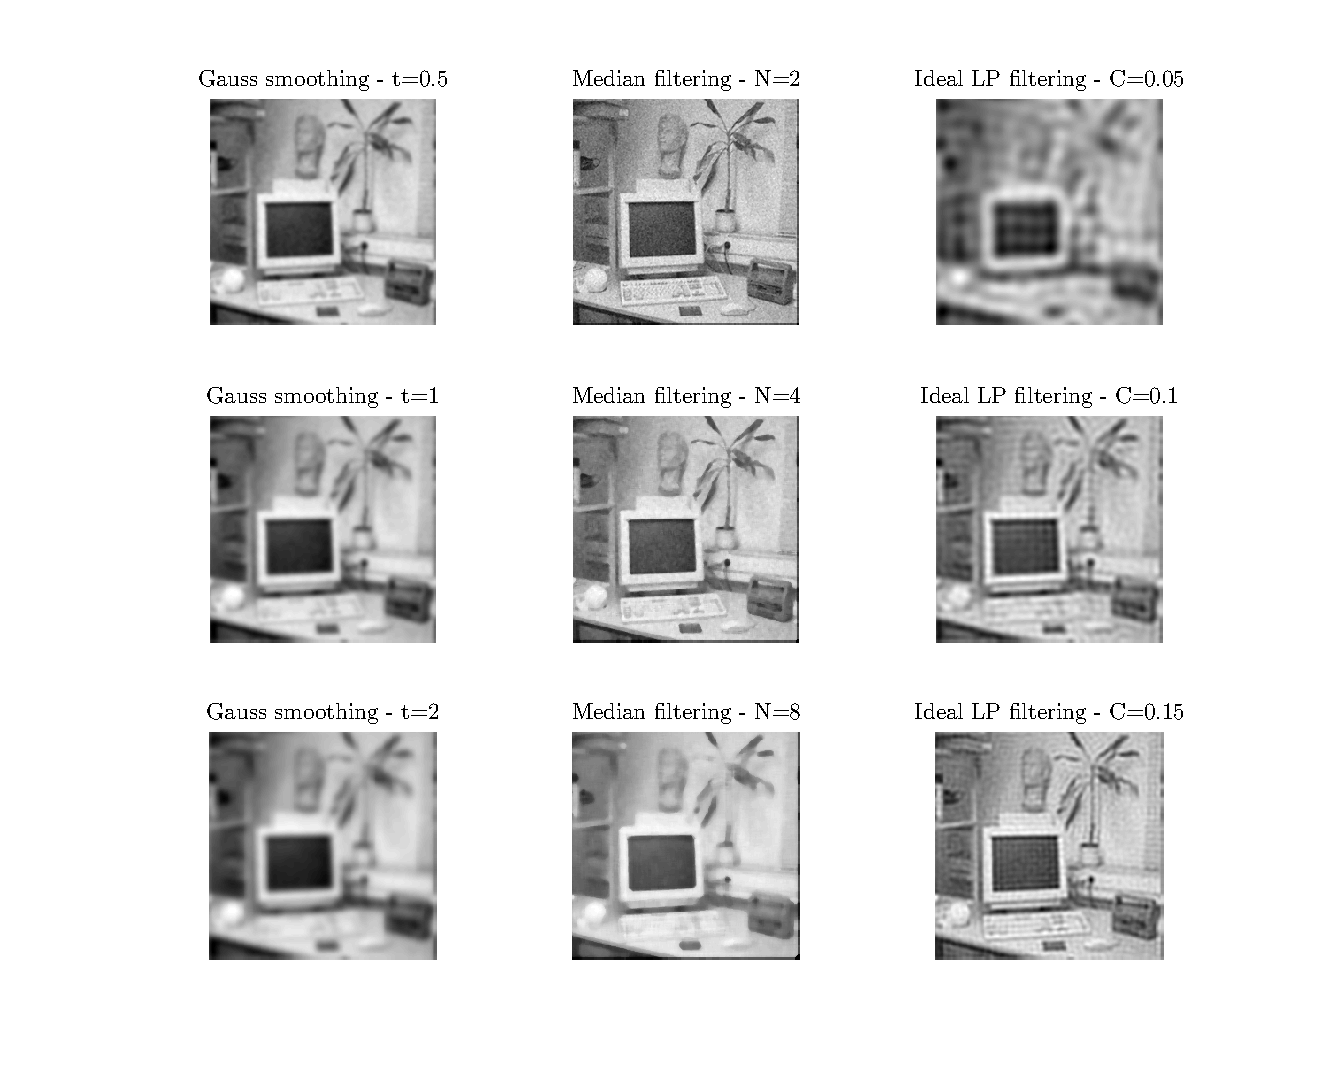
\includegraphics[width=\textwidth]{q17c}
 \caption{Image \texttt{office} plus added white Gaussian noise filtered with different methods and parameters.}
 \label{fig:q17c}
\end{figure}

\paragraph{Question 18: What conclusions can you draw from comparing the results of the respective
methods? Can you give a mathematical interpretation to explain the effects of each filter?}
There is not a filter that is best for noise reduction than any other. Depending on the characteristics of the noise some filters are better than others. The blur in the Gauss smoothing filter is due to the weighting of the frequency spectrum in which the lower frequencies are enhanced. The paint-like effect in the median filter is due to the algorithm itself which takes the median value of a set of neighbours around each pixel, eliminates the outliers. The ringing effect is due to the fact that an ideal filter in the frequency domain cannot be ideal in the spatial domain as it would require an infinite support. Alternatively, edges in which there is a change correspond in frequency to a wide spectrum across all frequencies, if we use only some of them Gibbs phenomenon appears producing this oscillations.

\paragraph{Question 19: What effects do you observe when subsampling the original image and the smoothed variants? Illustrate both filters with the best results found for iteration i = 4.}
When subsampling, the original image might have frequencies that cannot be represented anymore because they fall beyond the Nyquist frequency. If nothing is done, as in the images in the first row of Figure \ref{fig:q19a}, these frequencies are folded into the lower ones producing strange artifacts, aliasing. By smoothing the image before, the frequency content is limited so the subsampled image is free of artifacts due to aliasing, these can be seen in Figure \ref{fig:q19b} where the spectra of the images in previous figure are shown. For this two figures Gaussian smoothing has been used with \(t=20\). Figures \ref{fig:q19c} and \ref{fig:q19d} show the same for a smoothing done by an ideal LP filter with cutoff-frequency \(C=0.06\).

\begin{figure}[htbp]
 \centering
 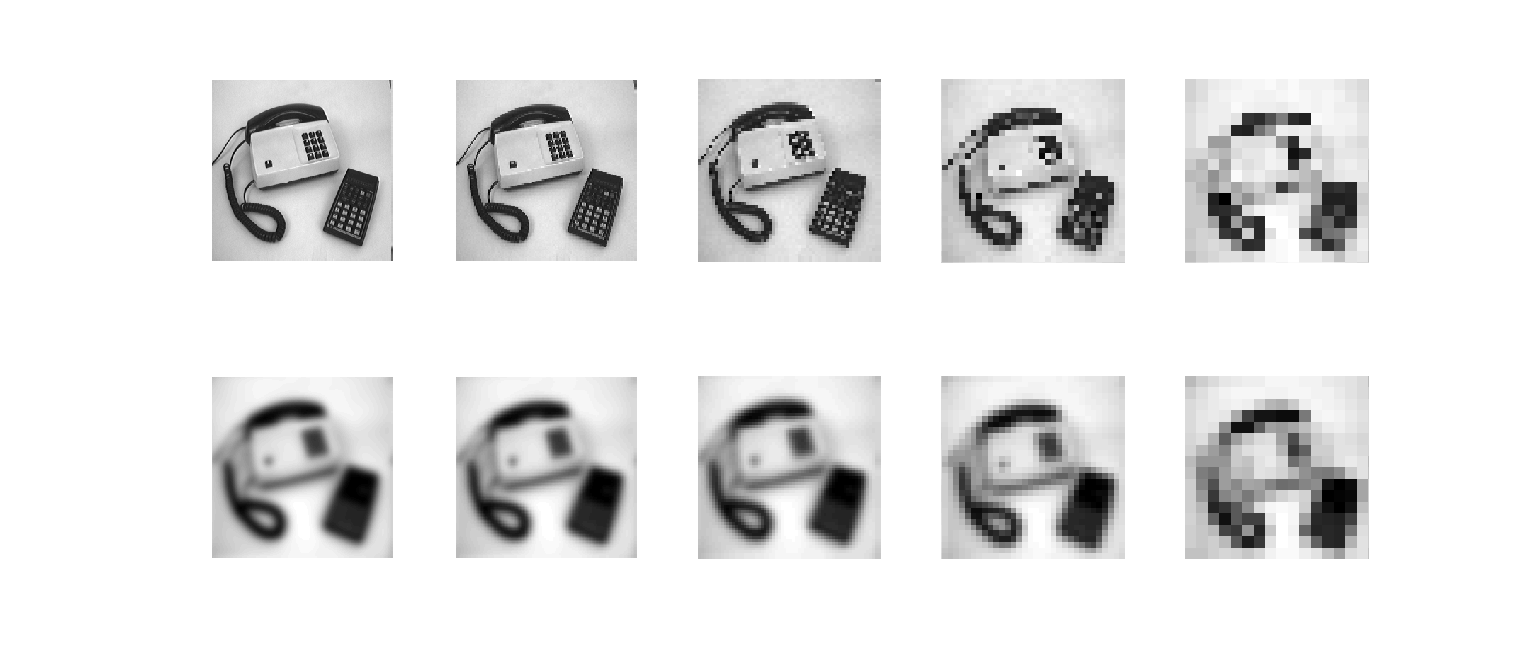
\includegraphics[width=\textwidth]{q19a}
 \caption{Image \texttt{phonecalc} subsampled and blurred with the Gaussian smoothing filter before subsampling.}
 \label{fig:q19a}
\end{figure}
\begin{figure}[htbp]
 \centering
 \includegraphics[width=\textwidth]{q19b}
 \caption{Spectra of image \texttt{phonecalc} subsampled and blurred with the Gaussian smoothing filter before subsampling.}
 \label{fig:q19b}
\end{figure}
\begin{figure}[htbp]
 \centering
 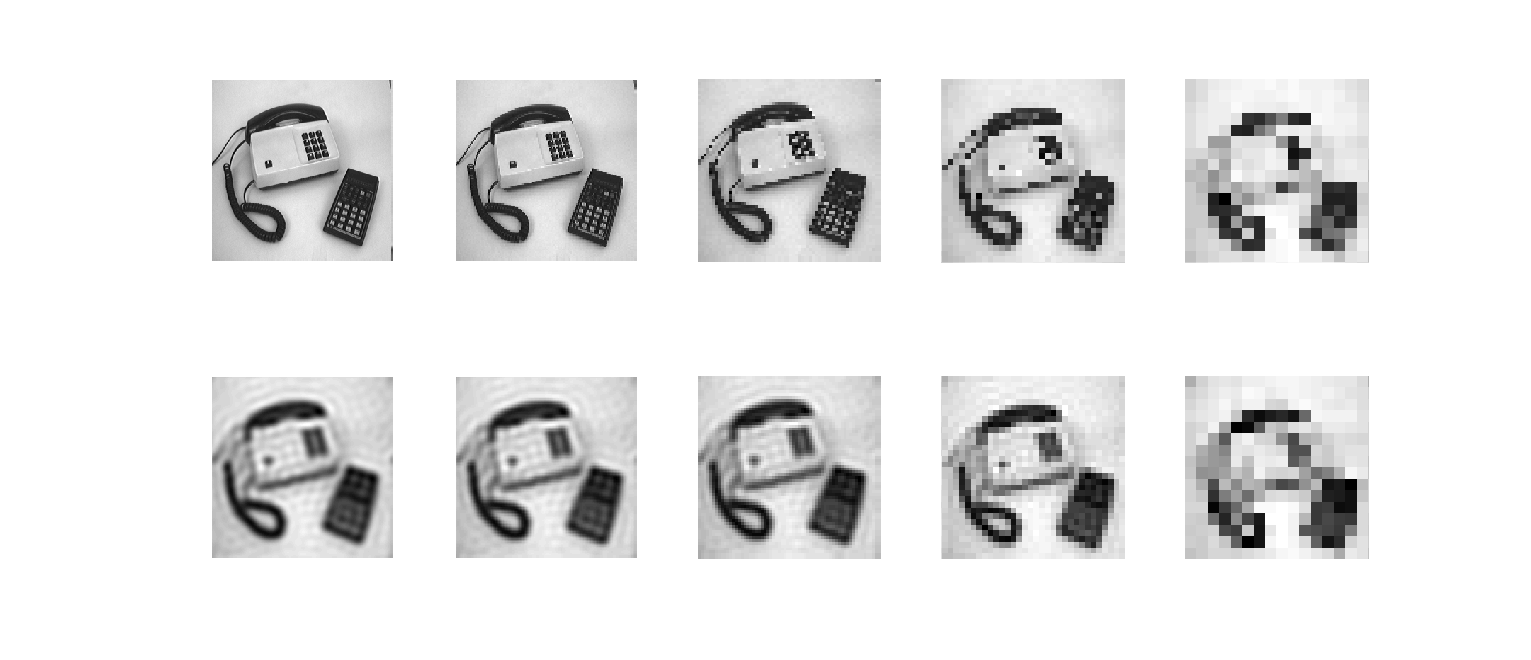
\includegraphics[width=\textwidth]{q19c}
 \caption{Image \texttt{phonecalc} subsampled and blurred with an ideal LP filter before subsampling.}
 \label{fig:q19c}
\end{figure}
\begin{figure}[htbp]
 \centering
 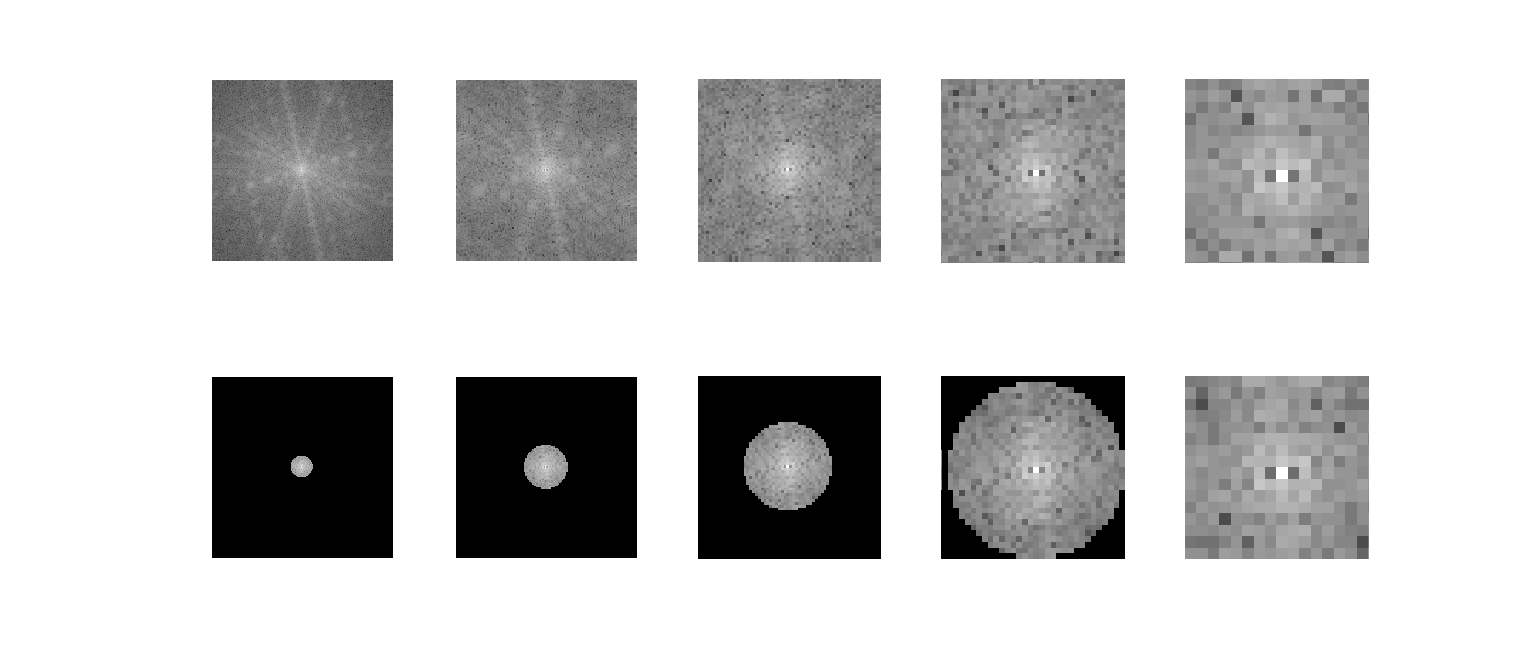
\includegraphics[width=\textwidth]{q19d}
 \caption{Spectra of image \texttt{phonecalc} subsampled and blurred with an ideal LP filter before subsampling.}
 \label{fig:q19d}
\end{figure}

\paragraph{Question 20: What conclusions can you draw regarding the effects of smoothing when combined with subsampling? Hint: think in terms of frequencies and side effects.}

As mentioned in previous question, smoothing allows limiting the frequency content of the image before subsampling so aliasing is avoided and no artifacts appear. However, the image is blurred so some narrow lines or edges are lost due to this fact. An example of that can be seen comparing subsampling iteration 4 in Figure \ref{fig:q19a}, where in the pre-blurred image there are no artifacts, but part of the telephone chord has almost vanished in the background.

%\section{Previous work}\label{previous work}
%A much longer \LaTeXe{} example was written by Gil~\cite{Gil:02}.
%
%\section{Results}\label{results}
%In this section we describe the results.
%
%\section{Conclusions}\label{conclusions}
%We worked hard, and achieved very little

\end{document}
This is never printed
